\chapter{影像动作放大技术概述}
\label{chap:previous}

根据视角的不同,现有的影像动作放大技术分为拉格朗日视角和欧拉视角两种视角。

拉格朗日视角和欧拉视角是流体动力学中研究流场的两种视
角\upcite{batchelor2000introduction}。其中,拉格朗日视角通过观察场景中一些独立的
粒子在时空中的运动轨迹来分析流体的运动;而欧拉视角则通过观察流体如何经过空间中一
个特定的位置来分析流体的运动。

\begin{definition}[拉格朗日视角的流体]
  在拉格朗日视角下,一个流体被定义为:$X(v,t)$,即粒子的运动轨迹向量$v$在$t$时刻
  的位置。
\end{definition}

\begin{definition}[欧拉视角的流体]
  在欧拉的视角下,一个流体被定义为:$V(x,t)$,即任意点$x$在$t$时刻的速度。
\end{definition}

两个定义有如下联系\upcite{lamb1993hydrodynamics}:
$$V(X(v,t),t)=\frac{\partial X}{\partial t}(v, t)$$,两边都表示一个粒子的运动轨迹$v$在$t$时刻的速度。

\section{拉格朗日视角的影像动作放大方法}
\label{sec:lagriangian}

2005年,文献\cite{liu2005motion}提出了一种拉格朗日视角的影像动作放大方法。方法包括如下几个步骤:

\begin{compactenum}
\item 视频校准。对视频的帧序列进行校准,以防止放大由于相机晃动而产生的动作。
\item 特征点轨迹聚类和流场插值。对特征点的轨迹进行聚类,得到$K$组动作的聚类。
  之后,对每帧图像的每个像素进行流场插值,得到稠密的流场。
\item 分割动作层。将每帧图像分割为$K$个动作层。
\item 放大用户选定的动作层。用户选定要放大的动作层后,对该层动作进行放大。
\item 渲染视频。重新渲染经过动作放大的视频。
\end{compactenum}

在放大动作信号前,需要先对视频的帧序列进行校准,以避免放大由于相机晃动而产生的动
作,并得到较为稳定的特征点。在这一步中,文献\cite{liu2005motion}主要采用了Sand等
人提出的视频校准算法\upcite{Sand2004}:首先,在初始参照帧中提取出不同尺度下的分
层Harris角点\upcite{lucas1981iterative,noble1989descriptions};其次,基于最小差
值平方和(Sum of Squared Differences, SSD)匹配,计算每个特征点从参照帧到其他帧的
流向量;随后,再利用局
部Lucas-Kanade算法\upcite{lucas1981iterative,shi1998motion}将这些流向量的精度优
化到亚像素级别;最后,根据这些流向量,计算出一个尽可能消除将所跟踪到的特征点的变
化的仿射变换矩阵,从而完成帧序列的校准。

% 假设从$K$帧图像跟踪和估计$N$个特征点,第$k$($k = 1\ldots k$) 帧中第$n$($n
% = 1\ldots N$)个特征点记为$(n,k)$,点$(n,k)$的坐标值记为$(x_{nk}, y_{nk})$,从参照帧到其他帧的流向量记为$(v_{nk}^{x}, v_{nk}^{y})$。

% 为了进行相似度估计,考虑一个大小为$2w\times 2w$的窗
% 口$B_{nk}$,而点$B_{nk}(p,q)$是在与$B_{nk}$的质心的相对坐标$(p,q)$处的点。
% 特征点$(n,k)$参与一个全局的仿射动作$A_{k}\in\mathbb{R}^{2\times 3}$的概率为:
% \begin{equation}
%   \label{eq:affine}
%   \mbox{Pr}_{nk}=exp\left\{-\left\|A_{k}[x_{nk} y_{nk} 1]^{T}]-[v_{nk}^{x}v_{nk}^{y}]^{T}\right\|^{2}/(2\sigma_{k}^{2})\right\}
% \end{equation}

% 其中,$\sigma_{k}$是平均重建误差
%$\sigma_{k}=\frac{1}{k}\sum_{n}\left\|A_{k}[x_{nk} y_{nk} 1]^{T}]-[v_{nk}^{x}v_{nk}^{y}]^{T}\right\|^{2}$

完成了视频的校准后,此时可以得到较为稳定的特征点。接下来再在每一帧中对第一帧中的
所有特征点进行第二次跟踪。跟踪过程同样包含特征点提取、SSD匹配及局部Lucas-Kanade
优化几个步骤。这一次特征点跟踪的目的是找到一组由可靠的特征点代表的动作轨迹。

根据同一个物理源产生的动作具有共变性和相同的共振频率的特
点\upcite{zelnik2003degeneracies},这些动作轨迹紧接着被传入一个聚类模块,以得到多
组动作的聚类。文献\cite{liu2005motion}使用归一化的相关系数(Normalized
Correlation)来度量轨迹的相关性。将一个特征点在水平和竖直方向上的速度分量$v^x$
和$v^y$组合为一个复值的动作向量$v^x + jv^y$,则一个轨迹中的两个特征
点$n$和$m$的归一化的动作相关指数$\rho_{n,m}$定义为:
\begin{equation}
  \label{eq:nomalized-correlation}
  \rho_{n,m}=\left|\frac{\sum_{k}(v_{nk}^{x}+jv_{nk}^{y})(v_{mk}^{x}+jv_{mk}^{y})}{\sqrt{(\sum_{k}(v_{nk}^x)^2+(v_{nk}^{y})^2)(\sum_{k}(v_{mk}^{x})^2+(v_{mk}^{y})^2}}\right|
\end{equation}

当两个特征点所标识的物体具有相互独立的动作时,使用公
式\ref{eq:nomalized-correlation}得到的归一化相关系数将趋于0。利用该度量手段,文
献\cite{liu2005motion}使用谱聚类(Spectral Clustering)算
法\upcite{shi1998motion}将所有轨迹聚类成$K$类,$K$为用户选定的一个数值。

完成了动作轨迹的聚类后,文献\cite{liu2005motion}使用一个两步插值算法对每帧图像
的每个像素进行插值:1) 使用局部加权线性回归方法\upcite{Sand2004}对每一
帧每隔3个像素点进行插值;2) 使用双三次差值方法再对每一帧的所有像素点进行插值。
经过这两步插值后,可以得到更稠密的流场。

接下来,文献\cite{liu2005motion}对上一步得到的流场使用Graph
Cuts算法\upcite{Boykov2001}将每帧图像分割成$K$组时空连续的动作层,这些动作层的
排序可以由人工确定,或根据遮挡情况确定\upcite{brostow1999motion}。当自动分割完成
后,还允许用户对分割结果进行人工编辑,去掉错误的像素,补上漏掉的像素。人工操作只
需在参照帧中进行。

完成动作层的分割后,用户选择要进行放大的动作层。每一帧该动作层的所有的像素的移动
距离都将乘以一个放大倍数。最后根据动作层的排序,从最底层渲染到最顶层,得到最终的视频结果。%该分割操作的本质是对
% 动作似然、颜色似然、空间连通性三个能量的最小化。这三个能量各自定义如下:

% \begin{definition}[动作似然]
%   第$k$帧的像素点$I_k(x,y)$属于第$l$层的动作似然为其重构误差:
%   \begin{equation}
%     \label{eq:prm}
%     Pr_{M}(l_k(x,y)|l)=exp{-\sum_{i=k-u}^{k+u}\frac{\left\|I_{k}(x,y)-I_{i}(M_{ik}^{(l)}(x,y))\right\|^{2}}{2\sigma_{M}^{2}}}
%   \end{equation}
% \end{definition}

% 其中,$u$为相邻帧的数量,$\sigma_{M}^{2}$为方差。

% \begin{definition}[颜色似然]
%   第$k$帧的像素点$I_k(x,y)$属于第$l$层的颜色似然为其高斯混合模型:
%   \begin{equation}
%     \label{eq:prm}
%     Pr_{M}(l_k(x,y)|l)=exp{-\sum_{i=k-u}^{k+u}\frac{\left\|I_{k}(x,y)-I_{i}(M_{ik}^{(l)}(x,y))\right\|^{2}}{2\sigma_{M}^{2}}}
%   \end{equation}
% \end{definition}

% \begin{equation}
%   \label{eq:total-energy}
%   \begin{aligned}
%     L^{*} =&{ arg }\min _{ L } -\sum _{ (x,y) } logPr_{ M }(I_{ k }(x,y)|L(x,y))\\
%   -&\xi \sum _{ (x,y) } logPr_{ C }(I_{ k }(x,y)|L(x,y))\\
%   +&\gamma \sum _{ (x,y) } \sum _{ (p,q)\in N_{ (x,y) } } V(I_{ k }(x,y),I_{ k }(x+p,y+q),L(x,y),L(x+p,y+q))
%   \end{aligned}
% \end{equation}

% 其中,

图\ref{fig:lag}总结了文献\cite{liu2005motion}的方法放大一个秋千的形变的过程。

\begin{figure}[htbp]
  \centering
  \subfloat[视频校准]{%
    \label{fig:lag-register-video}
    \includegraphics[width=.28\textwidth]{lag1.png}
  }\qquad
  \subfloat[特征点轨迹聚类]{%
    \label{fig:lag-cluster}
    \includegraphics[width=.28\textwidth]{lag2.png}
  }\qquad
  \subfloat[分割动作层]{%
    \label{fig:lag-layers}
    \includegraphics[width=.28\textwidth]{lag3.png}
  }\\
  \subfloat[直接放大(c)中秋千的动作层得到的结果(出现了空洞)]{%
    \label{fig:lag-motion-magnification}
    \includegraphics[width=.28\textwidth]{lag4.png}
  }\qquad
  \subfloat[对(d)进行背景填充得到的结果]{%
    \label{fig:lag-backgruond-fill}
    \includegraphics[width=.28\textwidth]{lag5.png}
  }\qquad
  \subfloat[先对(c)中秋千的动作层进行人工编辑再放大的结果]{%
    \label{fig:lag-modification}
    \includegraphics[width=.28\textwidth]{lag6.png}
  }
  \caption{拉格朗日视角的放大方法的处理流程}
  \label{fig:lag}
\end{figure}

图\ref{fig:liu}给出了使用文献\cite{liu2005motion}的方法对一个书架因受到按压
而发生的形变的放大结果。

\clearpage

\begin{figure}[htbp]
  \centering
  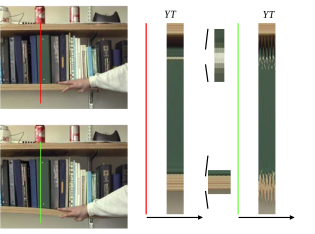
\includegraphics[width=.8\textwidth]{liu.pdf}
  \caption{使用拉格朗日视角的放大方法放大动作的结果}
  \label{fig:liu}
\end{figure}

拉格朗日视角的影像动作放大方法可以有效地从视频场景中找出微小的动作变化并进行放大。
然而,该方法存在以下几点不足:

\begin{compactenum}
\item 需要对特征点的运动轨迹进行精确的跟踪和估计。这个过程会耗费较多的计算资源。
\item 对特征点的跟踪容易受到遮挡的影响,从而影响跟踪结果。
\item 动作层分割的准确程度直接关系到最终的放大效果,而这个过程往往需要结合人工编
  辑才能达到理想的准确度,否则将导致放大结果出现空洞,需要在后期对图像进行背景
  填充等修补操作,这同样会增加算法的复杂度。
\end{compactenum}

\section{欧拉视角的影像动作放大方法}
\label{sec:eulerian}

欧拉视角的影像动作放大方法又被称为欧拉影像放大技术(Eulerian Video
Magnification, EVM)。2012 年,文献\cite{wu2012eulerian}提出了一种线性的欧拉影像动
作放大方法。其流程如下:

\begin{compactenum}
\item 空间域滤波。将视频序列进行金字塔多分辨率分解,得到不同空间频率的基带。
\item 频率滤波。对每个基带的图像进行频率域带通滤波,得到感兴趣的若干频带。
\item 动作放大。对带通滤波的结果进行线性放大。
\item 合成视频。合成经过放大后的图像。
\end{compactenum}

文献\cite{wu2012eulerian}的算法框架如图\ref{fig:linear}所示。

\begin{figure}[htbp]
  \centering
  \includegraphics[width=1.1\textwidth]{linear.pdf}
  \caption{线性的欧拉影像动作放大方法的算法框架图}
  \label{fig:linear}
\end{figure}

与拉格朗日视角的方法相比,欧拉视角的动作放大方法运算速度快,无需对放大后的结果进
行背景填充。除此之外,该方法不仅可以用来放大动作的变化,还可以用来放大颜色的变化。
图\ref{fig:color-motion}分別给出了使用文献\cite{wu2012eulerian}的方法放大动作和
颜色变化的结果,每一行右侧的图片代表视频中某条竖线的$YT$切片,该竖线的位置如图
\ref{fig:color-motion-original}中最左侧子图的绿线所示。

\begin{figure}[htbp]
  \centering
    \subfloat[输入视频及$YT$切片]{%
      \label{fig:color-motion-original}
      \includegraphics[height=2.5cm]{face2-1.png}~
      \includegraphics[height=2.5cm]{face2-3.png}~
      \includegraphics[height=2.5cm]{face2-4.png}~
      \includegraphics[height=2.5cm]{face2-5.png}\qquad
      \scalebox{4}[1]{\includegraphics[height=2.5cm]{face2-slice.png}}
    }\\
    \subfloat[动作变化放大结果及$YT$切片]{%
      \label{fig:color-motion-motion}
      \includegraphics[height=2.5cm]{face2-motion-2.png}~
      \includegraphics[height=2.5cm]{face2-motion-3.png}~
      \includegraphics[height=2.5cm]{face2-motion-4.png}~
      \includegraphics[height=2.5cm]{face2-motion-5.png}\qquad
      \scalebox{4}[1]{\includegraphics[height=2.5cm]{face2-motion-slice.png}}
      
    }\\
    \subfloat[颜色变化放大结果及$YT$切片]{%
      \label{fig:color-motion-color}
      \includegraphics[height=2.5cm]{face2-color-2.png}~
      \includegraphics[height=2.5cm]{face2-color-3.png}~
      \includegraphics[height=2.5cm]{face2-color-4.png}~
      \includegraphics[height=2.5cm]{face2-color-5.png}\qquad
      \scalebox{4}[1]{\includegraphics[height=2.5cm]{face2-color-slice.png}}
    }\\
  \caption{使用线性的欧拉影像动作放大方法放大动作变化和颜色变化的结果}
  \label{fig:color-motion}
\end{figure}

欧拉影像放大技术的第一步是对视频序列进行空间滤波。该过程主要借助拉普拉斯金字
塔\upcite{Burt1983},以分解得到不同的空间频率的基带。其原因有如下两点:

\begin{compactenum}
\item 有助于减少噪声。图像在不同空间频率下呈现出不同的信噪比(Signal to Noise
  Ratio, SNR)。空间频率越低,
  噪声越少,信噪比越高。因此,为了防止因放大噪声导致失真,可使用不同的放大倍数放
  大这些基带。最顶层的图像,即空间频率最低、信噪比最高的图像,可使用最大的放大倍
  数,下一层的放大倍数依次减小。
\item 便于对图像信号的逼近。空间频率较高的图像(如原视频图像)可能难以用泰勒级数
  展开来逼近。
\end{compactenum}

% 对视频序列的空间分解主要借助图像金字塔。如果要放大动作的变化,可以使用拉普拉斯金
% 字塔;如果要放大颜色的变化,则可以使用高斯金字塔。

得到不同空间频率的基带后,接下来需要对每一个基带进行频域的带通滤波,以得到感兴趣
的变化信号。

带通滤波器可以依据具体的应用来选择。窄通带的滤波器,如理想带通滤波器,可以直接截
取出感兴趣的频段,而避免放大其他频段,因而更适合用于需要对放大结果进行后续的时频
分析(例如提取心率、分析乐器的频率)的场合;宽通带的滤波器,如Butterworth带通滤波
器,二阶无限脉冲响应滤波器(Infinite Impulse Response Filter)等,可以更好的防止
振铃现象\cite{Gonzalez:2006:DIP:1076432},且更易于实现实时操作,因而更适合用在实
时性要求高,且不需要对放大结果进行时频分析的场合。

表\ref{tab:filters}列举了文献\cite{wu2012eulerian}处理face、guitar、subway及
wrist几个案例时所使用的滤波器。

\clearpage

\begin{table}[htbp]
  \centering
  \caption{文献\cite{wu2012eulerian}所使用的滤波器}
  \label{tab:filters}
  \begin{tabular}[c]{cccc}
    \toprule[1.5pt]
    案例名称 & 代表帧 & 滤波器示意图 \\
    \midrule
    face & \mgape{\includegraphics[height=3cm]{face.jpg}}
    & \mgape{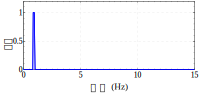
\includegraphics[height=3cm]{filter-face.pdf}} \\
    
    guitar & \mgape{\includegraphics[height=2.6cm]{guitar.jpg}} &
    \mgape{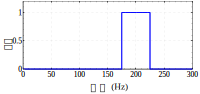
\includegraphics[height=3cm]{filter-guitar.pdf}}\\
    subway & \mgape{\includegraphics[height=3cm]{subway.jpg}} & 
    \mgape{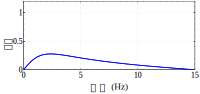
\includegraphics[height=3cm]{filter-subway.pdf}}\\
    wrist & \mgape{\includegraphics[height=3cm]{wrist.jpg}} &
    \mgape{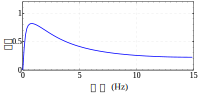
\includegraphics[height=3cm]{filter-wrist.pdf}}
    \\
    \bottomrule[1.5pt]
  \end{tabular}
\end{table}

文献\cite{wu2012eulerian}论证了带通滤波与感兴趣动作的关系:带通滤波的结果,就是对
感兴趣动作的逼近。

  以一维信号为例,设$I(x,t)$为点
$x$在$t$时刻的灰度值,且初始值为$f(x)$,则有:
\begin{equation}
  \label{eq:1}
  \left\{ \begin{aligned} I(x,t) & = f(x+\delta(t)) & , t >0 \\ I(x,0) & = f(x) &
        , t=0 \end{aligned} \right.
\end{equation}

其中,$\delta(t)$是变化信号。

要得到这个动作放大$\alpha$倍后的结果,就是要得到:

\begin{equation}
  \label{eq:2}
  \hat{I}(x,t)=f(x+(1+\alpha)\delta (t))
\end{equation}

为了将变化的部分分离出来,使用一阶泰勒级数展开来逼近公式\ref{eq:1}表示的动作:
\begin{equation}
  \label{eq:3}
  I(x,t)\approx f(x)+\delta(t)\frac{\partial f(x)}{\partial x}
\end{equation}

设上一步带通滤波的结果为$B(x,t)$,如果所有的变化信号$\delta(t)$的频率范围恰
好在带通滤波的频带范围之内,则有
\begin{equation}
  \label{eq:4}
  B(x,t)=\delta(t)\frac{\partial f(x)}{\partial x}
\end{equation}

对公式\ref{eq:2}所逼近的动作进行放大,就是将变化的部分乘以一个放大倍数
$\alpha$,再加回原来的信号中。即:
\begin{equation}
  \label{eq:5}
  \tilde{I}(x,t)=I(x,t)+\alpha B(x,t)
\end{equation}

联立公式\ref{eq:2}-\ref{eq:4},可得
\begin{equation}
  \label{eq:6}
  \tilde{I}(x,t)\approx f(x)+(1+\alpha)\delta(t)\frac{\partial f(x)}{\partial x}
\end{equation}

在这种情况下,$\tilde{I}(x,t)$约等于要求解的$I(x,t)$,即:
\begin{equation}
  \label{eq:7}
  \tilde{I}(x,t)\approx f(x+(1+\alpha)\delta(t))
\end{equation}

如果变化信号$\delta(t)$的频率范围超出了所选的频段范围。这种情况下,应用带通滤波
意味着只是保留了一部分的变化信号,而其他频率超出范围的信号将会被减弱。用$\gamma_k(t)$来表示在$t$时刻变化第$k$个变化信号减弱的倍数($0\le \gamma_k \le
1$),则有:
\begin{equation}
    \label{eq:8}
    B(x,t) = \sum_k \gamma_{k}\delta_{k}(t)\frac{\partial f(x)}{\partial x}
\end{equation}

此时,动作的放大可以用公式\ref{eq:9}表示:
\begin{equation}
  \label{eq:9}
  \tilde {I}(x,t)\approx f(x+\sum_k(1+\alpha_{k})\delta_{k}(t))
\end{equation}

其中,$\alpha_k$是$\alpha$与$\gamma_{k}$的乘积。

图\ref{fig:sinusoid}演示了对一个正弦信号的逼近和放大过程。

\begin{figure}[htbp]
  \centering
  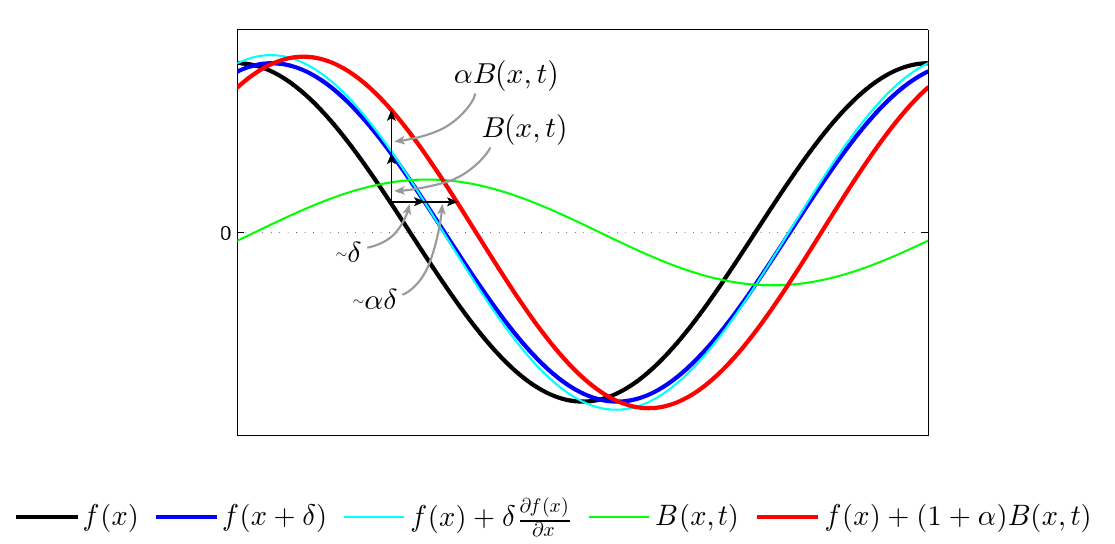
\includegraphics[width=\textwidth]{sinusoid.pdf}
  \caption{对一个正弦信号的逼近和放大过程}
  \label{fig:sinusoid}
\end{figure}

以上关于带通滤波结果与动作的关系结论是建立在相对平滑的图像和小的动作信号的假设上
的。对于空间频率较高的图像,使用泰勒级数逼近的结果会产生较大误差。文献
\cite{wu2012eulerian}给出了当前基带的空间频率$\omega$与放大倍数的界限值:
\begin{equation}
  \label{eq:bound1}
  (1+\alpha)\delta(t)<\frac{\lambda}{8}
\end{equation}

其中,$\lambda$是当前基带的空间波长,即$\lambda=\frac{\pi}{\omega}$。公式
\ref{eq:bound1}提供了计算每一层基带的合理放大倍数的准则。如图\ref{fig:guide}
所示,当$\alpha$达到该界限时,就维持在该界限值。

\clearpage

\begin{figure}[htbp]
  \centering
  \includegraphics[width=6.5cm]{guide.png}
  \caption{放大倍数$\alpha$的界限值}
  \label{fig:guide}
\end{figure}

线性的欧拉影像动作放大方法会在放大动作的同时放大噪声,所允许的放大倍数也较小。
2013年,文献\cite{Wadhwa2013PhaseBased}提出了一种基于相位的改进算法——首先使用抗混淆的复值可
控金字
塔
\upcite{portilla2000parametric,simoncelli1992shiftable,simoncelli1995steerable}来
进行多分辨率分解,并受到基于相位的光流
法\upcite{gautama2002phase,fleet1990computation,freeman1991motion}的启发,通过分
离和操纵滤波后信号的相位来调整动作的幅度。其流程如下:

\begin{compactenum}
\item 空间滤波。使用复值可控金字塔进行空间域分解,得到每个尺度、每个方向和位置的相位图。
\item 带通滤波。对每个尺度、每个方向和位置的信号进行带通滤波,得到感兴趣的若干频
  带,并去除直流分量。
\item 动作放大。放大带通滤波的结果。
\item 合成视频。合成经过放大的图像。
\end{compactenum}

基于相位的欧拉影像动作放大方法的算法框架如图\ref{fig:phase}所示。

\begin{figure}[htbp]
  \centering
  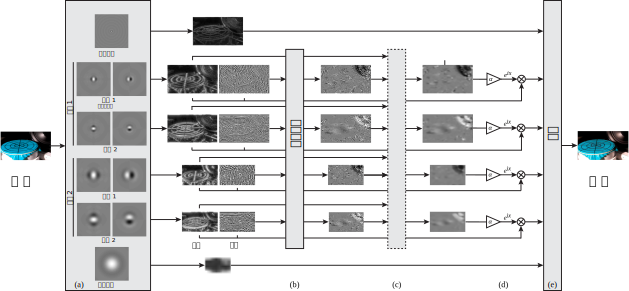
\includegraphics[width=1.1\textwidth]{phase.pdf}
  \caption{基于相位的欧拉影像动作放大方法的算法框架图}
  \label{fig:phase}
\end{figure}

基于相位的欧拉影像放大技术在放大动作的同时不会放大噪声,而是平移了噪声,因此允许
更大的放大倍数,其界限为
\begin{equation}
  \label{eq:bound2}
  a\delta(t)<\lambda \frac{n}{4}
\end{equation}

其中,$n$为复值可控金字塔的方向基带每个倍频程的滤波器数量。

图\ref{fig:compare}给出了分别使用两种方法放大一个吊车受风吹动产生的形变的结果对比。

\begin{figure}[htbp]
  \centering
  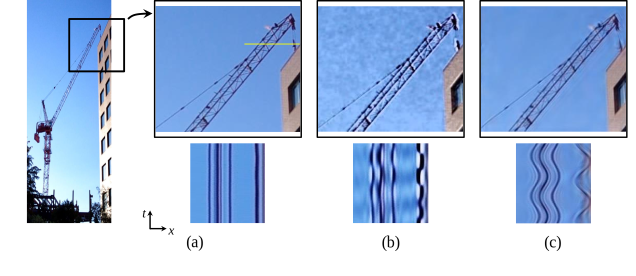
\includegraphics[width=\textwidth]{compare.pdf}
  \caption{线性的基于相位的欧拉影像放大方法的结果对比图。
    %(a) 顶部图:吊车的局部放大图。底部图:顶部图黄线区域的像素值随时
    %间变换的$XT$截面图。(b) 线性的方法的放大结果。噪声会连同吊车的动作一起被放
    %大,从而导致较大失真。(c) 基于相位的方法的放大结果,该方法在使用较大的放大倍
    %数时仍然不会引入较大噪声。
  }
  \label{fig:compare}
\end{figure}

欧拉影像动作放大方法的不足之处在于其分析的是整个场景中的感兴趣频段,对于存在大幅
度动作的场景,带通滤波的结果并不能反映真实的动作信息,此时的放大结果会产生明显
的“鬼影”现象,从而影响放大效果,如图\ref{fig:large-motion}所示。此外,对场景
中的非感兴趣区域的放大也会影响对放大结果的后继分析,如心率提取等。

\clearpage

\begin{figure}[htbp]
  \centering
  \subfloat[线性的方法]{%
      \includegraphics[width=.45\textwidth]{ghost-linear.png}
    }\qquad
   \subfloat[基于相位的方法]{%
      \includegraphics[width=.45\textwidth]{ghost-phase.png}
    }
  \caption{欧拉影像动作放大方法直接放大存在大幅度动作的场景会导致“鬼影”现象}
  \label{fig:large-motion}
\end{figure}

对于这个问题,文献\cite{Wadhwa2013PhaseBased}将相位的变化幅度超过一个阈值的动作
的放大倍数都设为0来避免对这些区域进行放大。如图\ref{fig:ignore}所示。

\begin{figure}[htbp]
  \centering
  \subfloat[直接全局放大结果,存在明显失真]{%
      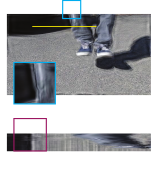
\includegraphics[width=.45\textwidth]{ignore.pdf}
    }~
   \subfloat[不对存在大幅度动作的物体进行放大]{%
      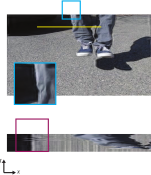
\includegraphics[width=.45\textwidth]{ignore2.pdf}
    }
  \caption{文献\cite{Wadhwa2013PhaseBased}通过避免放大存在大幅度动作的物体来防止失真}
  \label{fig:ignore}
\end{figure}

然而,这个方法直接忽略了存在大幅度动作的物体,因而无法对大幅度动作中的物体的细节
变化进行放大。而这类需求在实际生活中普遍存在,如放大一个移动中的人的脸部表情、颜
色变化等,显然上述的策略无法适应这类需求。

%%% Local Variables: 
%%% mode: latex
%%% TeX-master: "../thesis"
%%% End: 
